% !TeX root = ../main.tex
% Add the above to each chapter to make compiling the PDF easier in some editors.

\chapter{Evaluation}\label{chapter:evaluation}

The \glspl{holoassistapp} presented in \autoref{chapter:holoassistapps} already satisfy the main aim of this thesis project, which is to develop tools and workflows to easily create \gls{AR} experiences in a fixed-platform simulator (see \autoref{section:problemstatement}). \gls{holoassist} and its \gls{API} were able to address all the use cases encountered while developing those applications, and the resulting Python code was fairly concise and straightforward to write. Moreover, the process to draw a new mesh in Blender and to use the digital elevation model as a visual reference proved to be effective, and produced artifacts that were easy to integrate in a \gls{holoassistapp}. Although a formal evaluation of the usability of the \gls{API} and these workflows was not conducted, informal discussion with other researchers confirmed a general appreciation of the chosen design.

As part of this evaluation process for the \gls{holoassist} platform, a suite of augmentations for enhancing the landing experience at the Innsbruck airport has been developed. Besides being used to evaluate the \gls{API} flexibility, these augmentations have also been presented to some professional pilots, in order to gather their feedback on this initial attempt at an \gls{AR} integration within an aircraft simulator. Receiving a generally positive feedback would hint at \gls{AR} actually being useful in the cockpit, even if the currently developed augmentations fall short of the desired target. On the other side, receiving a more negative feedback could prompt a revision of the core assumptions of this project.

\section{Evaluating augmentations}\label{sect:evaluating_augmentations}

In order to evaluate the augmentations developed for the Innsbruck airport in a consistent way, it was decided to follow a partially standardized procedure.

It began with an introductory phase, in which the pilot was allowed to familiarize themselves with the Hololens and its main interaction paradigms, like using its hand detection feature to manipulate the position and scale of a virtual object. They also had to fill in the first part of a questionnaire, which focused on their flying experience and on their relationship with \gls{AR}/\gls{VR}.

After this introduction, the pilot was handed the \texttt{RNP-Y-RWY-08} approach chart for the Innsbruck airport (see \autoref{fig:lowi_approach_chart.png}), which showed the details of the maneuver that they would have to perform as part of the test. They were explicitly told that strictly following the procedure was not necessary and that they should consider it just as a general indication for the suggested approach, because the main focus of the test was on the user interface presented through the augmentations and not on the actual flight performance.

The pilot was then asked to land the aircraft at the Innsbruck airport by roughly following the given approach procedure and by using standard cockpit instrumentation. All pilots started from the same initial conditions. In particular, the visibility was reduced to $15$km, in order to increase the difficulty of the approach while still keeping it feasible to execute without using instrumental flight.

A few moments before touchdown, the simulation was paused and reset to initial conditions, in order to mitigate the stress that could be caused from a sub-optimal landing. After the reset the pilot was asked to wear the Hololens, which had already been configured with \gls{holoassist} running and the three \glspl{holoassistapp} designed for the Innsbruck airport shown. The pilot then had to fly the same approach again and land at the Innsbruck airport. While wearing the Hololens, pilots were explicitly told that they were free to rely on the augmentations that were shown, on the cockpit instrumentation or both. They were also asked to ignore hardware problems caused by the fact that the Hololens is still a research device, like its the weight, limited field of view and occasionally intense color aberration, as these problem will likely be solved by future versions of the \gls{HMD}.

The simulation was again interrupted a few moments before touchdown and the pilot was asked to fill in the second part of the questionnaire, which contained a structured comparison between the approach with and without the Hololens, and a few questions on the general applicability of \gls{AR} in aviation. In conclusion, a short open discussion in which the pilot was free to express any opinion they had on what they saw closed the test procedure, allowing for a more general and free-form kind of feedback to be expressed.

\section{Questionnaire results}

The \glspl{holoassistapp} developed for the Innsbruck airport have been shown to a small sample ($N=5$) of pilots, which experienced them following the evaluation procedure described in \autoref{sect:evaluating_augmentations}. The sample was composed mostly of amateur pilots with an amount of flight experience ranging from five to fifteen years and mostly focused on single engine planes and ultra-light aircrafts. Most of the sample was already familiar with \gls{VR} technologies, but had no previous experience with \gls{AR}. No symptoms of simulator sickness or of \gls{VR}/\gls{AR} sickness have been reported during or after the evaluation procedure.

The structured comparison between the approach with and without the Hololens consisted in a set of questions which had to be answered twice, once for each approach. The answer had to be given on a five-point Likert scale, ranging from \enquote{very easy} to \enquote{very difficult}. The results of this comparison are reported in tabular form in \autoref{table:questionnaire_part_two_results} and as a stacked bar chart in \autoref{fig:questionnaire_part_two_results_likert}. 

It can be observed that, overall, the approach with the Hololens was easier for the pilots, in particular regarding the estimation of the optimal trajectory. If only the questions regarding the correct approach path, turn radius and descent slope are considered, adding the Hololens yielded an improvement of around one level of the Likert scale: this means that the approach tunnel augmentation is fairly effective, and its appreciation was confirmed during the unstructured discussion. On the other side, the augmentation for the terrain surrounding the airport did not yield a significant benefit, and the unstructured discussion explained why: the visibility was still good enough to have a clear understanding of the terrain geometry, and augmenting it was superfluous. However, a quick test performed by one of the pilots suggests that in a situation with significantly worse visibility (around $100$m instead of $15$km), the terrain augmentation would instead be really useful.

The runway augmentation caused mixed reactions. Pilots agreed that from far away\footnote{One pilot put the threshold at $3$NM for the situation presented in this test.} the augmentation was useful to get a rough positioning of the runway, especially given that at the beginning of the approach it was occluded by a mountain and without the augmentation pilots could only guess its location. However, as the airplane moved closer to it, the misalignment between the real runway and the augmented one caused significant confusion and degraded the experience. This misalignment was caused\footnote{Unfortunately, the root cause for this misalignment has been identified and fixed only after gathering the pilots feedback. The version of \gls{holoassist} described in this document already includes these fixes.} by the difficulty of correctly locating the \gls{PEP} for the projection setup and by the instability of the position estimate made by the Hololens \gls{API} for the QR codes. Besides completely fixing the alignment issue (which has already been significantly improved), another suggested solution was to have the runway augmentation disappear once the airplane is closer than a certain distance threshold (dependent on the current visibility conditions).

The last part of the questionnaire was designed to gauge the pilot's opinion on the applicability of \gls{AR} to aviation in general, and its results are shown in \autoref{fig:questionnaire_part_two_results_general_questions}. These questions show that in conditions of lower visibility pilots would definitely appreciate the help offered by the Hololens, but they would not use it if the sky is clear. They would like to have \gls{AR} capabilities integrated in the aircraft models they usually fly and in general think that \gls{AR} has the potential to improve the instrumentation commonly available in commercial airplanes. However, the unstructured discussion highlighted that, although the Hololens could be a desirable addition to the standard instrumentation, it does not seem sufficient to entirely replace it.


\begin{table}
  \centering
  \begin{tabular}{c c c c c c c c} 
    \toprule
        \makecell{How difficult\\was it to\ldots} & & Pilot A & Pilot B & Pilot C & Pilot D & Pilot E & avg. \\
    \midrule
        \multirowcell{3}{\ldots estimate the\\distance of\\the terrain?} & w.   & 1 & 1 & 2 & 3 & 1 & \\
                            & w/o. & 2 & 1 & 1 & 3 & 1 & \\
                            & imp. & 1 & 0 & -1 & 0 & 0 & 0\\
    \midrule
        \multirowcell{3}{\ldots estimate\\your altitude?} & w.   & 2 & 1 & 2 & 2 & 1 & \\
                            & w/o. & 2 & 1 & 1 & 4 & 1 & \\
                            & imp. & 0 & 0 & -1 & 2 & 0 & 0.2\\
    \midrule
        \multirowcell{3}{\ldots estimate the\\position of\\the runway?} & w.   & 2 & 1 & - & 2 & 2 & \\
                            & w/o. & 1 & 2 & - & 3 & 4 & \\
                            & imp. & -1 & 1 & - & 1 & 2 & 0.75\\
    \midrule
        \multirowcell{3}{\ldots estimate the\\correct approach\\path?} & w.   & 1 & 1 & 1 & 1 & 1 & \\
                            & w/o. & 2 & 2 & 3 & 2 & 3 & \\
                            & imp. & 1 & 1 & 2 & 1 & 2 & 1.4\\
    \midrule
        \multirowcell{3}{\ldots estimate the\\turn radius of\\the last curve?} & w.   & 1 & 1 & 1 & 1 & 1 & \\
                            & w/o. & 3 & 1 & 2 & 3 & 1 & \\
                            & imp. & 2 & 0 & 1 & 2 & 0 & 1\\
    \midrule
        \multirowcell{3}{\ldots estimate the\\correct descent\\slope?} & w.   & 1 & 1 & 2 & 1 & 1 & \\
                            & w/o. & 1 & 2 & 3 & 3 & 1 & \\
                            & imp. & 0 & 1 & 1 & 2 & 0 & 0.8\\
    \midrule
        \multirowcell{3}{\ldots maintain the\\correct speed\\and altitude? } & w.   & 1 & 1 & 2 & 3 & 1 & \\
                            & w/o. & 3 & 1 & 3 & 3 & 1 & \\
                            & imp. & 2 & 0 & 1 & 0 & 0 & 0.6\\
    \midrule
        \multicolumn{2}{c}{average improvement} & 0.71 & 0.43 & 0.50 & 1.14 & 0.57 &\\
    \bottomrule
  \end{tabular}
  \caption{Results of the structured comparison between the approach with and without the Hololens. The table reports the reply that each pilot gave on a five-point Likert scale ranging from \enquote{1 (very easy)} to \enquote{5 (very difficult)}. The table also reports the improvement that each pilot perceived after wearing the Hololens, computed as the difference between the score reported without (\enquote{w/o.}) the \gls{HMD} and with it (\enquote{w.}): a negative improvement means that wearing the Hololens worsened the pilot experience. The last column shows the average improvement across all pilots for a given question, whereas the last row shows the average improvement across all questions for a given pilot.}\label{table:questionnaire_part_two_results}
\end{table}

\begin{figure}[p]
  \centering
  %https://tex.stackexchange.com/questions/411920/labels-on-a-grouped-and-stacked-bar-chart
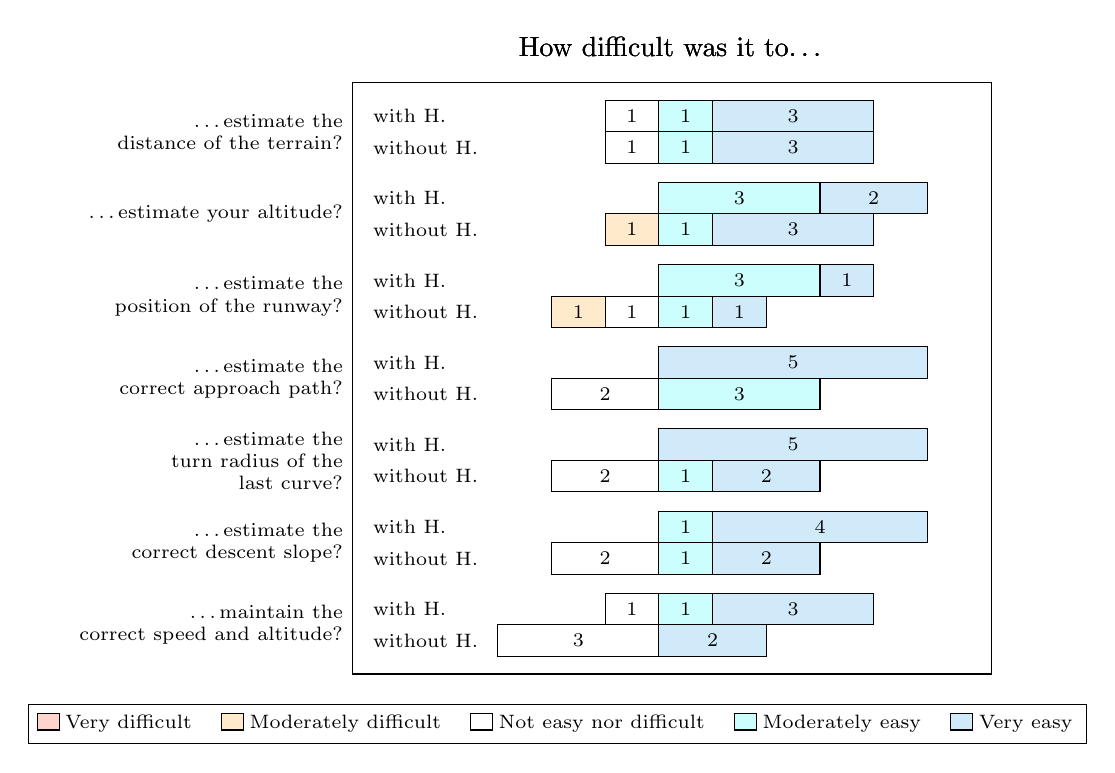
\begin{tikzpicture}[
    %every node/.style=draw,
    %every label/.style=draw
]
    \definecolor{myred}{RGB}{218,32,0}
    \definecolor{myredfill}{RGB}{255,212,204}
    \definecolor{myorange}{RGB}{255,153,0}
    \definecolor{myorangefill}{RGB}{255,235,204}
    \definecolor{mygreen}{RGB}{0,184,0}
    \definecolor{mygreenfill}{RGB}{202,255,202}
    \definecolor{mycyan}{RGB}{5,154,199}
    \definecolor{mycyanfill}{RGB}{205,254,254}
    \definecolor{myblue}{RGB}{13,98,153}
    \definecolor{mybluefill}{RGB}{208,234,250}

    \pgfplotsset{
        every axis/.style={
            xbar stacked,
            width=0.8\textwidth,
            height=0.75\textwidth,
            bar width=4mm,
            title={How difficult was it to\ldots},
            %symbolic y coords = {Q1,Q2,Q3},
            ytick = {0, 1, 2, 3, 4, 5, 6},
            yticklabels = {
                \ldots maintain the\\correct speed and altitude?,
                \ldots estimate the\\correct descent slope?,
                \ldots estimate the\\turn radius of the\\last curve?,
                \ldots estimate the\\correct approach path?,
                \ldots estimate the\\position of the runway?,
                \ldots estimate your altitude?,
                \ldots estimate the\\distance of the terrain?
            },
            yticklabel style={font=\scriptsize, align=right},
            ytick style = {draw = none},
            xtick = \empty,
            xmin=-4, xmax=4.5,
            enlarge y limits=0.1,
            enlarge x limits=0.2,
            legend style={
                at={(0.32,-0.05)},
                anchor=north,
                legend columns=5,
                /tikz/every even column/.append style={column sep=0.3cm},
                font=\scriptsize
            },
            nodes near coords,
            nodes near coords style={font=\scriptsize, align=center},
            point meta=explicit symbolic,
            % extra x ticks={0},
            % extra x tick style={
            %     grid style={black},
            %     xticklabel=\empty,
            % },
        }    
    }

    \begin{axis}[bar shift = 2mm, yticklabels={}]
        \addplot+[xbar, black, fill=white] plot coordinates {
            (-1,6) [1]
            (0,5) [0]
            (0,4) [0]
            (0,3) [0]
            (0,2) [0]
            (0,1) [0]
            (-1,0) [1]
        };
        \addplot+[xbar, black, fill=myorangefill] plot coordinates {
            (0,6) [0]
            (0,5) [0]
            (0,4) [0]
            (0,3) [0]
            (0,2) [0]
            (0,1) [0]
            (0,0) [0]
        };
        \addplot+[xbar, black, fill=myredfill] plot coordinates {
            (0,6) [0]
            (0,5) [0]
            (0,4) [0]
            (0,3) [0]
            (0,2) [0]
            (0,1) [0]
            (0,0) [0]
        };
        \addplot+[xbar, black, fill=mycyanfill] plot coordinates {
            (1,6) [1]
            (3,5) [3]
            (3,4) [3]
            (0,3) [0]
            (0,2) [0]
            (1,1) [1]
            (1,0) [1]
        };
        \addplot+[xbar, black, fill=mybluefill] plot coordinates {
            (3,6) [3]
            (2,5) [2]
            (1,4) [1]
            (5,3) [5]
            (5,2) [5]
            (4,1) [4]
            (3,0) [3]
        };

        \node[right,yshift=2mm] at (-5.5, 0) {\scriptsize with H.};
        \node[right,yshift=2mm] at (-5.5, 1) {\scriptsize with H.};
        \node[right,yshift=2mm] at (-5.5, 2) {\scriptsize with H.};
        \node[right,yshift=2mm] at (-5.5, 3) {\scriptsize with H.};
        \node[right,yshift=2mm] at (-5.5, 4) {\scriptsize with H.};
        \node[right,yshift=2mm] at (-5.5, 5) {\scriptsize with H.};
        \node[right,yshift=2mm] at (-5.5, 6) {\scriptsize with H.};
    \end{axis}

    \begin{axis}[bar shift = -2mm]
        \addplot+[xbar, black, fill=myredfill] plot coordinates {
            (0,6) [0]
            (0,5) [0]
            (0,4) [0]
            (0,3) [0]
            (0,2) [0]
            (0,1) [0]
            (0,0) [0]
        };
        \addplot+[xbar, black, fill=white] plot coordinates {
            (-1,6) [1]
            (0,5) [0]
            (-1,4) [1]
            (-2,3) [2]
            (-2,2) [2]
            (-2,1) [2]
            (-3,0) [3]
        };
        \addplot+[xbar, black, fill=myorangefill] plot coordinates {
            (0,6) [0]
            (-1,5) [1]
            (-1,4) [1]
            (0,3) [0]
            (0,2) [0]
            (0,1) [0]
            (0,0) [0]
        };
        \addplot+[xbar, black, fill=mycyanfill] plot coordinates {
            (1,6) [1]
            (1,5) [1]
            (1,4) [1]
            (3,3) [3]
            (1,2) [1]
            (1,1) [1]
            (0,0) [0]
        };
        \addplot+[xbar, black, fill=mybluefill] plot coordinates {
            (3,6) [3]
            (3,5) [3]
            (1,4) [1]
            (0,3) [0]
            (2,2) [2]
            (2,1) [2]
            (2,0) [2]
        };
        \node[right,yshift=-2mm] at (-5.5, 0) {\scriptsize without H.};
        \node[right,yshift=-2mm] at (-5.5, 1) {\scriptsize without H.};
        \node[right,yshift=-2mm] at (-5.5, 2) {\scriptsize without H.};
        \node[right,yshift=-2mm] at (-5.5, 3) {\scriptsize without H.};
        \node[right,yshift=-2mm] at (-5.5, 4) {\scriptsize without H.};
        \node[right,yshift=-2mm] at (-5.5, 5) {\scriptsize without H.};
        \node[right,yshift=-2mm] at (-5.5, 6) {\scriptsize without H.};
        %\legend{Very difficult, Not easy nor difficult, Moderately difficult, Moderately easy, Very easy}
    \end{axis}

    \begin{axis}[ytick = \empty]
        \addplot+[xbar, black, fill=myredfill] plot coordinates {
            (0,0) [0]
        };
        \addplot+[xbar, black, fill=myorangefill] plot coordinates {
            (0,0) [0]
        };
        \addplot+[xbar, black, fill=white] plot coordinates {
            (0,0) [0]
        };
        \addplot+[xbar, black, fill=mycyanfill] plot coordinates {
            (0,0) [0]
        };
        \addplot+[xbar, black, fill=mybluefill] plot coordinates {
            (0,0) [0]
        };
        \legend{Very difficult, Moderately difficult, Not easy nor difficult, Moderately easy, Very easy}
    \end{axis}


\end{tikzpicture}
  \caption{Results of the structured comparison between the approach with and without the Hololens. The plot shows how many pilots replied in a certain way to a certain question. The sample size is too small for this plot to be really effective, but it still shows that on average replies to questions regarding the approach without the Hololens tend to be slightly more shifted towards the \enquote{very difficult} side than replies to questions regarding the approach with the Hololens.}\label{fig:questionnaire_part_two_results_likert}
\end{figure}


\begin{figure}
  \centering
  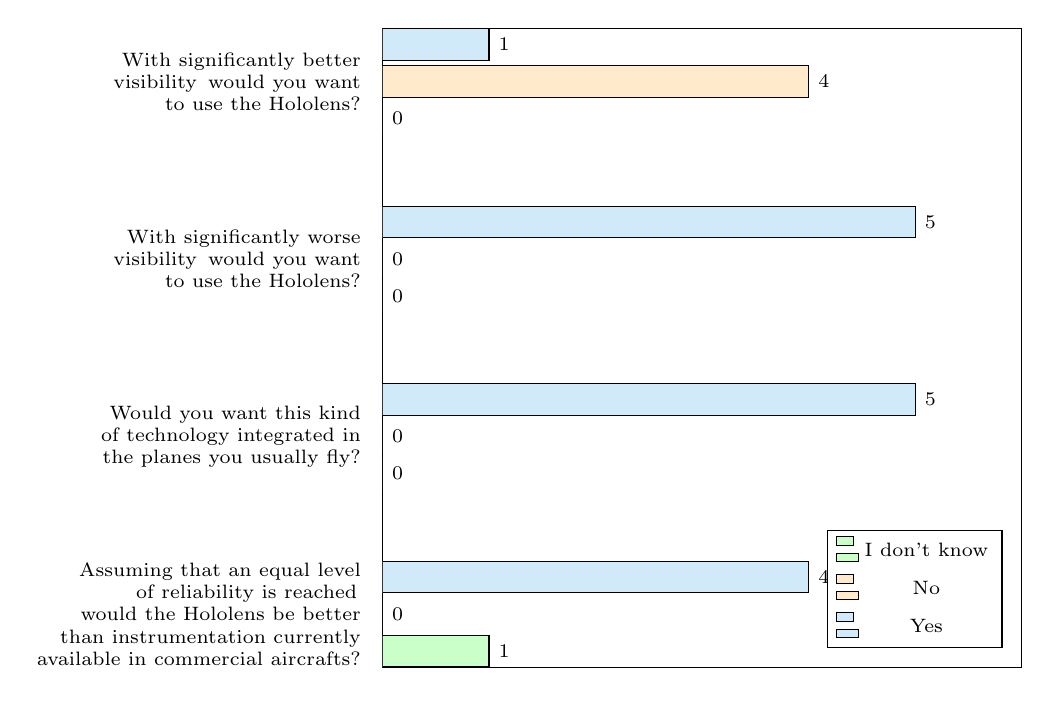
\begin{tikzpicture}
    \definecolor{myred}{RGB}{218,32,0}
    \definecolor{myredfill}{RGB}{255,212,204}
    \definecolor{myorange}{RGB}{255,153,0}
    \definecolor{myorangefill}{RGB}{255,235,204}
    \definecolor{mygreen}{RGB}{0,184,0}
    \definecolor{mygreenfill}{RGB}{202,255,202}
    \definecolor{mycyan}{RGB}{5,154,199}
    \definecolor{mycyanfill}{RGB}{206,241,253}
    \definecolor{myblue}{RGB}{13,98,153}
    \definecolor{mybluefill}{RGB}{208,234,250}

    \pgfplotsset{
        every axis/.style={
            width=0.8\textwidth,
            height=0.8\textwidth,
            xbar, xmin=0, xmax=6,
            bar width=4mm,
            ytick = {0, 1, 2, 3},
            yticklabels = {
                Assuming that an equal level\\of reliability is reached\,\\would the Hololens be better\\than instrumentation currently\\available in commercial aircrafts?,
                Would you want this kind\\of technology integrated in\\the planes you usually fly?,
                With significantly worse\\visibility\, would you want\\to use the Hololens?,
                With significantly better\\visibility\, would you want\\to use the Hololens?,
            },
            yticklabel style={font=\scriptsize, align=right},
            ytick style = {draw = none},
            xtick = \empty,
            nodes near coords,
            nodes near coords style={font=\scriptsize},
            legend pos = south east,
            legend style={
                font=\scriptsize,
                row sep=1mm
            },
        }    
    }

    \begin{axis}
        \addplot+[black, fill=mygreenfill] coordinates {
            (0, 3)
            (0, 2)
            (0, 1)
            (1, 0)
        };
        \addplot+[black, fill=myorangefill] coordinates {
            (4, 3)
            (0, 2)
            (0, 1)
            (0, 0)
        };
        \addplot+[black, fill=mybluefill] coordinates {
            (1, 3)
            (5, 2)
            (5, 1)
            (4, 0)
        };
        \legend{I don't know, No, Yes}
    \end{axis}

\end{tikzpicture}
  \caption{Results of the general questions asked to pilots regarding their opinion on the more general applicability of \gls{AR} to aviation.}\label{fig:questionnaire_part_two_results_general_questions}
\end{figure}

\section{Further remarks}\label{sec:final_remarks}

Besides the results reported above, a few more elements worth mentioning emerged during the various unstructured discussions.

One of the pilots included in the sample happened to also be a flight instructor and pointed out how relevant the usage of the Hololens to display an approach trajectory could be for new pilots during training. Further investigation in this space is definitely warranted. Another pilot pointed out that sometimes, especially for flights under visual metereological conditions (VMC), the approach trajectory is not always fixed and standardized: this means that the way in which the approach tunnel has been computed for this test might not be applicable to all situations.

Almost all of the interviewed pilots expressed the desire to include some elements of the primary flight display in the Hololens itself, in particular as far as speed, vertical speed, altitude and flight path marker are concerned. Since this was an almost universal request, its implementation should definitely be prioritized in future works.

Pilots were also asked for their opinion about the integration of Hololens-like systems in \glspl{eVTOL}, and the replies were mixed. Although there seems to be potential in such kind of integration, there is also the risk of overwhelming inexperienced pilots with too much information and with the complexity of the new interface. Just copying elements like speed, altitude and flight path marker from the standard primary flight display to an \gls{AR} \gls{HMD} would not be sufficient, and a more thoughtful analysis that takes into account also the capabilities of the flight controller is required. Besides approach path tunnels, other suggested visualizations for \glspl{eVTOL} include the highlighting of obstacles (which would be particularly useful in an urban environment) and visualizing the trajectory that the \gls{eVTOL} will follow during flight configuration transitions (e.g. when transitioning from vertical flight to horizontal flight). In particular, this second aspect is quite relevant, as visually determining the point in space at which such a transition is complete is not trivial. A final suggestion, useful in the case of vertical landing, would be to have an augmentation showing the landing area at the current altitude of the \gls{eVTOL}: in this case, the pilot would not have to align the aircraft with a landing pad of the ground, which is probably difficult to look at, but could just look around at its current height level.

In conclusion, pilots were asked if they had ideas for other augmentations that could be shown during the Innsbruck approach. In no particular order, they suggested to:

\begin{enumerate}
    \item Add an augmentation that shows the distance to the current target (e.g.\ to the runway). Such an augmentation could look like quest markers in video-games, appearing above the current target and displaying the distance from it in an appropriately scaled font;
    \item Add an augmentation that integrates \gls{TCAS} information to highlight the position of other planes directly in the pilots field of view;
    \item Extend the terrain augmentation by using color to signal which part of the terrain cannot be out-climbed with the current aircraft performance. For example, if the airplane is too close to a specific terrain feature to out-climb it before reaching it, that part of the terrain would be colored in red;
    \item Add an augmentation that extends the center line of the runway, so that the pilot would more clearly see how they should align the airplane for the landing. This augmentation should also interact with the terrain surrounding the airport, for example by being properly occluded by the mountains;
    \item Add an augmentation that uses arrows to signal wind direction and intensity in the area surrounding the current airplane position.
\end{enumerate}